\let\negmedspace\undefined
\let\negthickspace\undefined
\documentclass[journal]{IEEEtran}
\usepackage[a5paper, margin=10mm, onecolumn]{geometry}
%\usepackage{lmodern} % Ensure lmodern is loaded for pdflatex
\usepackage{tfrupee} % Include tfrupee package
\setlength{\headheight}{1cm} % Set the height of the header box
\setlength{\headsep}{0mm}     % Set the distance between the header box and the top of the text
\usepackage{gvv-book}
\usepackage{gvv}
\usepackage{cite}
\usepackage{amsmath,amssymb,amsfonts,amsthm}
\usepackage{algorithmic}
\usepackage{graphicx}
\usepackage{textcomp}
\usepackage{xcolor}
\usepackage{txfonts}
\usepackage{listings}
\usepackage{enumitem}
\usepackage{mathtools}
\usepackage{gensymb}
\usepackage{comment}
\usepackage[breaklinks=true]{hyperref}
\usepackage{tkz-euclide} 
\usepackage{listings}
% \usepackage{gvv}                                        
\def\inputGnumericTable{}                                 
\usepackage[latin1]{inputenc}                                
\usepackage{color}                                            
\usepackage{array}                                            
\usepackage{longtable}                                       
\usepackage{calc}                                             
\usepackage{multirow}                                         
\usepackage{hhline}                                           
\usepackage{ifthen}                                           
\usepackage{lscape}
\begin{document}

\bibliographystyle{IEEEtran}
\vspace{3cm}
\parindent 0px

\title{6.6.11}
\author{EE24BTECH11050 - Pothuri Rahul}
% \maketitle
% \newpage
% \bigskip
{\let\newpage\relax\maketitle}

\renewcommand{\thefigure}{\theenumi}
\renewcommand{\thetable}{\theenumi}
\setlength{\intextsep}{10pt} % Space between text and floats


\numberwithin{equation}{enumi}
\numberwithin{figure}{enumi}
\renewcommand{\thetable}{\theenumi}

\textbf{Question :} \\ 
If 4-digit numbers greater than 5,000 are randomly formed from the digits 0,1,3,5,7 . What is the probability of forming a number divisible by 5 when the digits are repeated.
\solution \\
\textbf{Theoretical solution:}
Let A,B,C and D be the digits of four digited number ABCD . \\
S be the set containing four digit numbers formed with 0,1,3,5,7 that are greater than 5000. \\
No.of values A can take - 2 (5,7) \\
No.of values B can take - 5 (0,1,3,5,7) \\
No.of values C can take - 5 (0,1,3,5,7) \\
No.of values D can take - 5 (0,1,3,5,7) \\
Total no.of numbers can be formed = 2 x 5 x 5 x 5 = 250 \\
But the number 5000 is included in this set (A=5, B=0, C=0, D=0) . \\
n(s) = 250 - 1 $\implies$ n(s) = 249 .

E be the set containing the four digit numbers formed with 0,1,3,5,7 that are greater than 5000 and divisible by 5. \\
No.of values A can take - 2 (5,7) \\
No.of values B can take - 5 (0,1,3,5,7) \\
No.of values C can take - 5 (0,1,3,5,7) \\
No.of values D can take - 2 (0,5) \\
Total no.of numbers can be formed = 2 x 5 x 5 x 2 = 1000 \\
But the number 5000 is included in this set (A=5, B=0, C=0, D=0) . \\
n(E) = 100 - 1 $\implies$ n(s) = 99 .
\begin{align*}
Probability = \frac{n(s)}{n(E)} \\
Probability = \frac{99}{249}
\end{align*}
\textbf{Simulation} \\
\begin{enumerate}
\item Let us randomly get the numbers formed by 0,1,3,5,7 and greater than 5000. 
\item Run this loop for large no.of times i.e., n(s) .
\item Count the number of times a multiple of 5 comes i.e., n(E) .
\item Now required probability is $\frac{n(E)}{n(s)}$  
\item Run this iteration large no.of times so that we get probability of each times and the most repeated one is closest value of the required probability.
\end{enumerate}
The simulated one is not exactly equal to that of the theoretical one because the outcomes dare not equally likely, where we consider outcomes to be equally likely in theoretical solution . \\
The plot below shows the no.of times the particular probability repeats.

\begin{figure}[htbp] % Positioning options: here, top, bottom, page
    \centering
    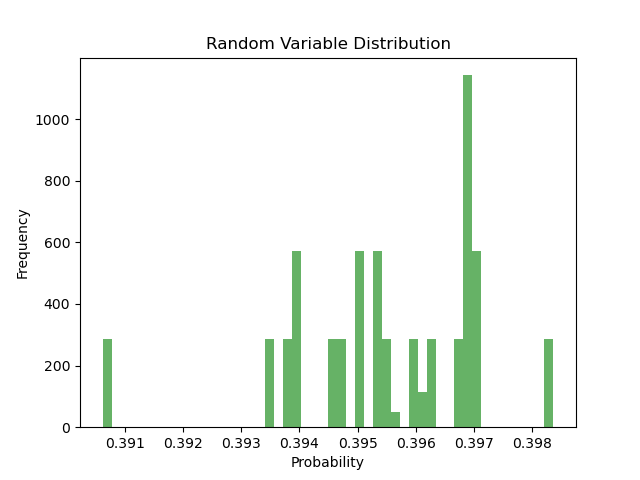
\includegraphics[width=\textwidth]{fig/plot.png} % Replace "filename" with your image file
    \caption{Plot}
\end{figure}



From the plot above , probability is nearly 0.397 which is nearly equal to the theoretical value. i.e., $\frac{99}{249}$ .  



\end{document}
